\documentclass{gnulike}
\usepackage{natbib}
\usepackage{graphics}
\usepackage{chngcntr}
\usepackage{sectsty}
\usepackage{rotating}
\usepackage{emptypage}
\usepackage[titletoc]{appendix}

\let\leqslant=\leq


\newcommand{\psm}{small-scale physical modeling method}
\newcommand{\bialt}{\textit{BiAlt} }
\newcommand{\cmnt}[1]{}



\definecolor{light-gray}{gray}{0.95}
\definecolor{bashgray}{RGB}{209,214,217}
\newcommand{\addbash}[1]{
	\begin{center}
	\colorbox{bashgray}{\begin{minipage}{0.9\textwidth}
  	\ttfamily \$ #1
\end{minipage}}
	\end{center}
}


\usepackage[dvipsnames]{xcolor}
\usepackage{minibox}

\usepackage{graphicx}
\usepackage{color}

\definecolor{vibrisblue1}{RGB}{90,151,190}
\definecolor{vibrisblue2}{RGB}{25,96,177}

\newcommand{\subtitle}{FDPSV}

\titleformat{\chapter}[hang] 
{\normalfont\huge\bfseries}{\thechapter}{0.5em}{} 
\titlespacing*{\chapter}{0pt}{-20pt}{20pt}

\usepackage{makeidx}
\makeindex

\mdseries

\begin{document}

\begin{titlepage}
  \newpage
  \null
  \vskip 10.0em
  \let\center\flushleft
  {\noindent \huge{\bf FDPSV} \par}
  \vskip -0.5em
  {\noindent \rule{\textwidth}{0.3em} \par}

  {\hfill Documentation for FDPSV version 0.1 \par}
  
  {\hfill 11 January 2017 \par}
  
  \vfill
  
  {\noindent \Large{Damien Pageot}}
  \vskip -0.5em
  {\noindent \rule{\textwidth}{0.2em} \par}
  \vskip 1.0cm
\end{titlepage}

% ----------------------------------------------------------------------
% MANUAL LICENSE
% ----------------------------------------------------------------------
\null\vfill
\pagenumbering{gobble}
\noindent Copyright \copyright\ 2016-2017 Damien Pageot.\\

\noindent Permission is granted to copy, distribute and/or modify this document under the terms of the GNU Free Documentation License, Version 1.3 or any later version published by the Free Software Foundation; with no Invariant Sections, no Front-Cover Texts, and no Back-Cover Texts. A copy of the license is included in the section entitled "GNU Free Documentation License".
\clearpage\newpage

% ----------------------------------------------------------------------
% TABLE OF CONTENTS
% ----------------------------------------------------------------------
\pagenumbering{roman}
\tableofcontents
\thispagestyle{empty}
\clearpage\newpage

\pagenumbering{arabic}
% ----------------------------------------------------------------------
% INTRODUCTION
% ----------------------------------------------------------------------
\chapter{Introduction}
\index{Introduction}

% ----------------------------------------------------------------------
% THEORETICAL BACKGROUND
% ----------------------------------------------------------------------
\chapter{Theoretical background}

\section{Equation of motion}
\index{equation of motion}

\section{Staggered grid}
\index{staggered grid}

\cite{virieux1986psv,levander1988fourth}

\begin{figure}[!ht]
  \centering
  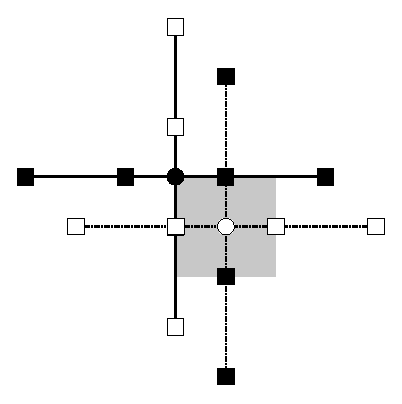
\includegraphics[width=8cm]{fig/staggered.eps}
\end{figure}

\noindent Second order forward ($D^{+}$) and backward ($D^{-}$) operators:
\index{forward operator}
\index{backward operator}
\begin{eqnarray}
  D^{+}=f(i+1)-f(i) \nonumber \\
  D^{-}=f(i)-f(i-1)
\end{eqnarray}

\noindent Fourth order forward ($D^{+}$) and backward ($D^{-}$) operators:
\begin{eqnarray}
  D^{+}=c_{1}[f(i+1)-f(i)]+c_{2}[f(i+2)-f(i-1)] \nonumber \\
  D^{-}=c_{1}[f(i)-f(i-1)]+c_{2}[f(i+1)-f(i-2)]
\end{eqnarray}

\index{Lam\'e parameters}
\begin{eqnarray}
  \bar{\mu}(i+\frac{1}{2}, j+\frac{1}{2})=\frac{1}{4}(\mu(i,j)+\mu(i+1,j)+\mu(i,j+1)+\mu(i+1,j+1) \\
  \rho_{x}(i,j+\frac{1}{2}) = \frac{1}{2}(\rho (i,j+1)+\rho(i,j)) \\
  \rho_{z}(i+\frac{1}{2},j) = \frac{1}{2}(\rho (i+1,j)+\rho(i,j))
\end{eqnarray}

\section{Initial and boundary conditions}
\index{absorbing boundary condition}
\index{free surface condition}

\cite{berenger1994perfectly}

% ----------------------------------------------------------------------
% GETTING STARTED
% ----------------------------------------------------------------------
\chapter{Getting started}

\section{Requirements}

\noindent For FDPSV program:
\begin{itemize}
	\item GNU make $>=$ 4.1
	\item GNU gfortran $>=$ 4.4/4.7
\end{itemize}

\noindent Optional for examples:
\begin{itemize}
	\item python $>=$ 2.7
	\item python-numpy $>=$ 1.8.2
\end{itemize}

\noindent Optional:
\begin{itemize}
	\item Seismic Un*x $>=$ 43R1
\end{itemize}

\subsection{Compilation}
\addbash{make}

% ----------------------------------------------------------------------
% INPUT PARAMETERS AND FILES
% ----------------------------------------------------------------------
\section{Input parameters and files}
\index{input parameters}
\index{input files}

% ----------------------------------------------------------------------
% NUMERICAL EXAMPLES
% ----------------------------------------------------------------------
\chapter{Numerical examples}

\begin{appendices}
% ----------------------------------------------------------------------
% APPENDICES
% ----------------------------------------------------------------------
%\appendix
%\addappheadtotoc
%\chapter{GNU Free Documentation License}
\input{fdl-1.3}

\end{appendices}
  
% ----------------------------------------------------------------------
% References
% ----------------------------------------------------------------------

\bibliography{references}

\clearpage
\newpage
\thispagestyle{empty}
\printindex

\end{document}
